%%%%%%%%%%%%%%%%%%%%%%%%%%%%%%%%%%%%%%%%%
% FRI Data Science_report LaTeX Template
% Version 1.0 (28/1/2020)
% 
% Jure Demšar (jure.demsar@fri.uni-lj.si)
%
% Based on MicromouseSymp article template by:
% Mathias Legrand (legrand.mathias@gmail.com) 
% With extensive modifications by:
% Antonio Valente (antonio.luis.valente@gmail.com)
%
% License:
% CC BY-NC-SA 3.0 (http://creativecommons.org/licenses/by-nc-sa/3.0/)
%
%%%%%%%%%%%%%%%%%%%%%%%%%%%%%%%%%%%%%%%%%


%----------------------------------------------------------------------------------------
%	PACKAGES AND OTHER DOCUMENT CONFIGURATIONS
%----------------------------------------------------------------------------------------
\documentclass[fleqn,moreauthors,10pt]{ds_report}
\usepackage[english]{babel}

\graphicspath{{fig/}}




%----------------------------------------------------------------------------------------
%	ARTICLE INFORMATION
%----------------------------------------------------------------------------------------

% Header
\JournalInfo{FRI Natural language processing course 2024}

% Interim or final report
\Archive{Project report} 
%\Archive{Final report} 

% Article title
\PaperTitle{Conversations with Characters in Stories for Literacy}

% Authors (student competitors) and their info
\Authors{Žan Kogovšek, Žiga Drab, Vid Cesar}

% Advisors
\affiliation{\textit{Advisors: Slavko Žitnik}}

% Keywords
\Keywords{Literacy Improvement, Dialogue Agents, Harry Potter Dialogue Dataset, Pre-trained Language Models}
\newcommand{\keywordname}{Keywords}


%----------------------------------------------------------------------------------------
%	ABSTRACT
%----------------------------------------------------------------------------------------
% Abstract
\Abstract{
In addressing the challenge of declining literacy interest among youth, we examine the use of character-driven chatbots for educational enhancement, aiming to make reading more engaging. We explore related works and existing NLM-based services, highlighting their strengths in user engagement and identifying inaccuracies in content representation. Our future work involves developing a framework for generating and evaluating such chatbots, with a focus on accuracy, engagement, and educational value.
}

%----------------------------------------------------------------------------------------

\begin{document}

% Makes all text pages the same height
\flushbottom 

% Print the title and abstract box
\maketitle 

% Removes page numbering from the first page
% \thispagestyle{empty} 
%----------------------------------------------------------------------------------------
%	ARTICLE CONTENTS
%----------------------------------------------------------------------------------------

\section*{Introduction}

The diminishing interest in reading among young individuals and their struggle with high-level literacy skills present a significant challenge to their academic and professional success \cite{murray2021literacy}. Given literacy's crucial role, innovative methods are needed to motivate the young to engage with literature.

One possible solution is through the innovative use of chatbots. The research conducted by Brandtzaeg et al. \cite{why_chatbots} highlights that one of the primary reasons for the adoption of chatbots lies in their entertainment value. This finding suggests that chatbots serve not just as tools for information retrieval or customer service, but also as platforms for entertainment.

Lately, the evolution of open-domain conversation models, Adiwardana et al. \cite{adiwardana2020towards}, has achieved remarkable progress, uncovering the possibility of human-like sensibleness in machine conversations. Models can overcome the limitations of simple exchanges by incorporating traits commonly found in real-life interactions, such as emotion \cite{zhou2018emotional} and empathy \cite{rashkin2018towards_empathy}. This approach, often referred to as style-controlling conversation models, significantly enhances the quality of engagement, making the conversation feel more genuine and relatable \cite{smith2020controlling}. Zhang et al. \cite{zhang2018personalizing} introduce a model capable of producing responses with consistent personalities by utilizing personal descriptions, a step forward in making conversation models more personalized and engaging.

In this paper, we explore the potential of enhancing children's literacy through entertaining chatbots with personalities, modeled after characters from literature. Our objective is to develop a streamlined pipeline capable of generating chatbots across various datasets, thereby enabling children to interact with their favorite figures and make reading more appealing.

\section*{Related Work}
Enhancing children's literacy through technology and innovative approaches has been already explored by Nielen et al. \cite{nielen2018digital}. They introduced a pedagogical agent, an animated mouse guiding fifth graders in their reading. This agent boosted reading motivation and vocabulary learning by engaging them with summaries and reflective questions. 

Moving on to personalized dialogue agents, Chen et al. \cite{chen2023large} introduced the Harry Potter Dialogue (HPD) dataset, which contains not only dialogues but also background information, including scenes, speakers and their relationship with Harry. They evaluated LLMs, like Alpaca, ChatGPT and GPT-3 on the HPD dataset through fine-tuning and in-context learning. Results indicate significant potential for improvements, yet the dataset proves useful in steering models towards more accurately reflecting Harry Potter's character.

Han et al. \cite{han2022meet} introduce a strategy, Pseudo Dialog Prompting (PDP), that utilizes statements from various characters alongside a pre-trained language model to generate conversations. Among the pre-trained models selected for this purpose are GPT-2-XL, GPT-J, and GPT-Neo. The performance of these models was tested both through automatic evaluation using MaUdE and via human assessments. The findings from these experiments demonstrate that the PDP strategy successfully crafts responses that accurately mirror the style of the specified characters.

Figure~\ref{fig:generic_framework} presents a generic framework demonstrated by Hefny et al. \cite{generic_framework} for creating character-based chatbots structured around five modules. These include the conversational user interface, entities, intents, webhook, and database. The conversational user interface serves as the initial point of interaction, allowing users to input prompts and select entities. Following this, the system loads the chosen entity and attempts to understand the user's intent. This intent is then processed through a webhook module, which facilitates access to the database. From here, responses are randomly selected and presented to the user

\begin{figure}[ht]
        \centering 
	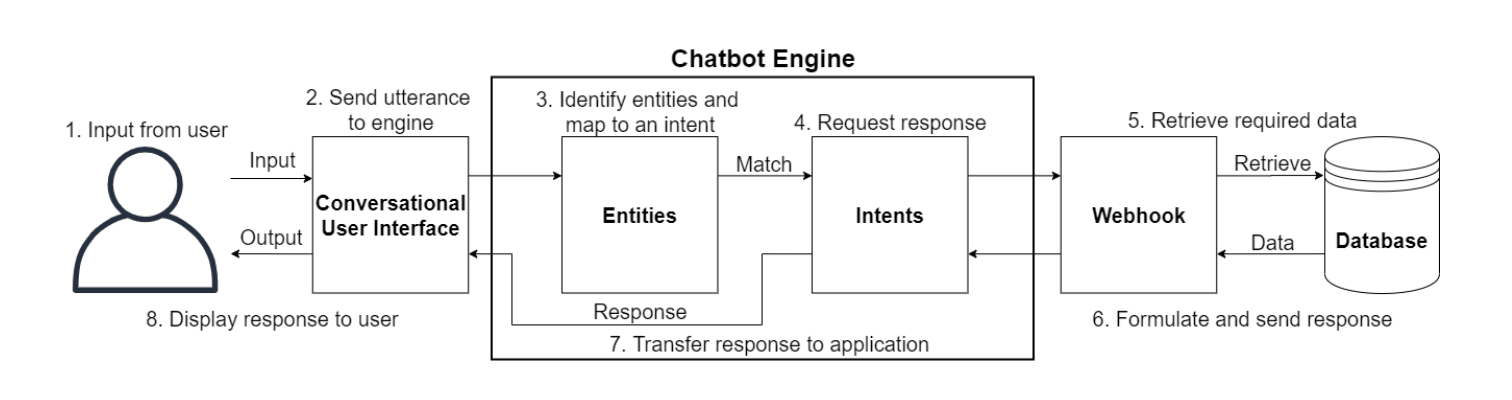
\includegraphics[width=\linewidth]{fig/general_framework_from_article.png}
	\caption{\textbf{Proposed generic framework} for building character-based chatbots \cite{generic_framework}.}
	\label{fig:generic_framework}
\end{figure}

\section*{Bot Persona Services}

We tested Character.ai, a service offering interactive dialog agents based on Neural Language Models (NLM) for entertainment. We began a conversation with Greek Mythology hero Achilles (\href{https://character.ai/chat/EBMwCtvGQWrCk_xeglpGWfQiCJOCkGu7PMWbEWLINlY}{Version 1 Achilles}). 
The responses generated were not just the responses of a character, but also included his actions - "nodding slowly" for example, and even interpretation of said actions - "expression full of sadness and regret". The model was reluctant to give out information about himself, which he deemed important, and was trying to find out what we knew about him. When faced with direct questions about something, it seemed as if it was trying to avoid answering it - maybe because of the character's nature. Testing the model further, we noticed incorrectness in story of his death. Despite repeated inquiries, the model persisted with the incorrect narrative, highlighting concerns over its handling of basic factual accuracy. 

We also tried another model of the same character. While avoiding the previous error, it inaccurately identified Achilles' parents, mistaking his father for a god and his mother for a human. The model again struggled with factual accuracy. Despite a disclaimer on Character.ai indicating that responses are fictional, the inaccuracies observed in the models' responses raise concerns about factual correctness.

For improving literacy, some dialog agents can be used as they use rich vocabulary and there is a lot of extra text in addition to the answer itself. Yet, some agents provide extremely short answers. Example of such dialog agent is Miles Morales (\href{ttps://character.ai/chat/KfUosnPgcC9hoTWbJq_2z1cQi-719T8cldRLa2fTb1Y}{Version 1 Miles Morales}), where even information about character actions and context is very sparse, indicating not all agents are effective for literacy improvement. Model descriptions, using terms like "cold" or "rude," can also guide the selection of agents supportive to literacy goals.

\section*{Initial Idea}
    Adapting the generic framework for constructing character-based chatbots, we simplify it by removing the database and webhook modules. These are replaced with an existing model capable of generating responses to prompts in real time. Our revised framework retains a user interface that enables users to select their preferred entity. Additionally, an entity selector is employed to choose the suitable character model from the character model pool. The architecture of our updated framework is illustrated in Figure~\ref{fig:application_diagram}.

\begin{figure}[ht]
        \centering 
	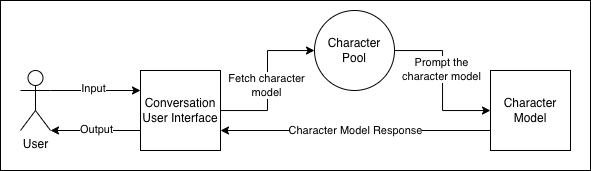
\includegraphics[width=\linewidth]{fig/Character_Chatbot_Pipeline.drawio.png}
	\caption{\textbf{Adapted generic framework} for constructing character-based chatbots with 3 modules.}
	\label{fig:application_diagram}
\end{figure}

    Our framework requires a diverse collection of character models, comprising the character model pool. The process for assembling this pool is detailed in Figure~\ref{fig:chatbot_pipeline}. Initially, the dataset pool will include the Harry Potter dataset mentioned earlier, with plans to expand it with additional datasets. The Pre-Trained Model pool will feature GPT-2 models, as discussed in the related works and will also include the Llama pre-trained model if possible. These datasets and pre-trained models will be merged through supervised fine-tuning to create character-specific models, which are then gathered in the character model pool. Given the complexity of these pre-trained models, which consist of billions of parameters, the creation and management of multiple character chatbots will necessitate the use of high-performance computing resources.

\begin{figure}[ht]
        \centering 
	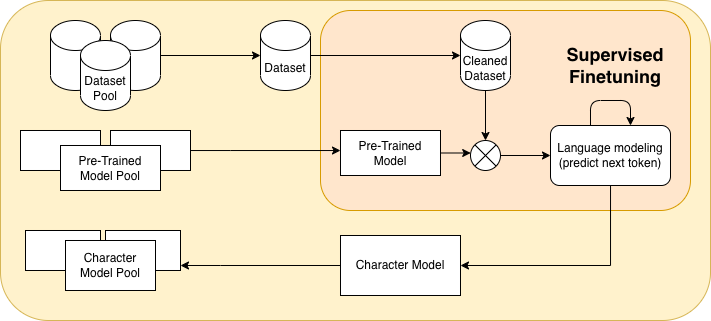
\includegraphics[width=\linewidth]{fig/Character_Model_Pipeline.drawio.png}
	\caption{\textbf{Character Model Pool Pipeline} with supervised finetuning.}
	\label{fig:chatbot_pipeline}
\end{figure}

%------------------------------------------------
% UNCOMMENT SELECTED LINE USING: "CTRL+ /"

% \section*{Methods}

% Use the Methods section to describe what you did an how you did it -- in what way did you prepare the data, what algorithms did you use, how did you test various solutions ... Provide all the required details for a reproduction of your work.

% Below are \LaTeX examples of some common elements that you will probably need when writing your report (e.g. figures, equations, lists, code examples ...).


% \subsection*{Equations}

% You can write equations inline, e.g. $\cos\pi=-1$, $E = m \cdot c^2$ and $\alpha$, or you can include them as separate objects. The Bayes’s rule is stated mathematically as:

% \begin{equation}
% 	P(A|B) = \frac{P(B|A)P(A)}{P(B)},
% 	\label{eq:bayes}
% \end{equation} 

% where $A$ and $B$ are some events. You can also reference it -- the equation \ref{eq:bayes} describes the Bayes's rule.

% \subsection*{Lists}

% We can insert numbered and bullet lists:

% % the [noitemsep] option makes the list more compact
% \begin{enumerate}[noitemsep] 
% 	\item First item in the list.
% 	\item Second item in the list.
% 	\item Third item in the list.
% \end{enumerate}

% \begin{itemize}[noitemsep] 
% 	\item First item in the list.
% 	\item Second item in the list.
% 	\item Third item in the list.
% \end{itemize}

% We can use the description environment to define or describe key terms and phrases.

% \begin{description}
% 	\item[Word] What is a word?.
% 	\item[Concept] What is a concept?
% 	\item[Idea] What is an idea?
% \end{description}


% \subsection*{Random text}

% This text is inserted only to make this template look more like a proper report. Lorem ipsum dolor sit amet, consectetur adipiscing elit. Etiam blandit dictum facilisis. Lorem ipsum dolor sit amet, consectetur adipiscing elit. Interdum et malesuada fames ac ante ipsum primis in faucibus. Etiam convallis tellus velit, quis ornare ipsum aliquam id. Maecenas tempus mauris sit amet libero elementum eleifend. Nulla nunc orci, consectetur non consequat ac, consequat non nisl. Aenean vitae dui nec ex fringilla malesuada. Proin elit libero, faucibus eget neque quis, condimentum laoreet urna. Etiam at nunc quis felis pulvinar dignissim. Phasellus turpis turpis, vestibulum eget imperdiet in, molestie eget neque. Curabitur quis ante sed nunc varius dictum non quis nisl. Donec nec lobortis velit. Ut cursus, libero efficitur dictum imperdiet, odio mi fermentum dui, id vulputate metus velit sit amet risus. Nulla vel volutpat elit. Mauris ex erat, pulvinar ac accumsan sit amet, ultrices sit amet turpis.

% Phasellus in ligula nunc. Vivamus sem lorem, malesuada sed pretium quis, varius convallis lectus. Quisque in risus nec lectus lobortis gravida non a sem. Quisque et vestibulum sem, vel mollis dolor. Nullam ante ex, scelerisque ac efficitur vel, rhoncus quis lectus. Pellentesque scelerisque efficitur purus in faucibus. Maecenas vestibulum vulputate nisl sed vestibulum. Nullam varius turpis in hendrerit posuere.


% \subsection*{Figures}

% You can insert figures that span over the whole page, or over just a single column. The first one, \figurename~\ref{fig:column}, is an example of a figure that spans only across one of the two columns in the report.

% \begin{figure}[ht]\centering
% 	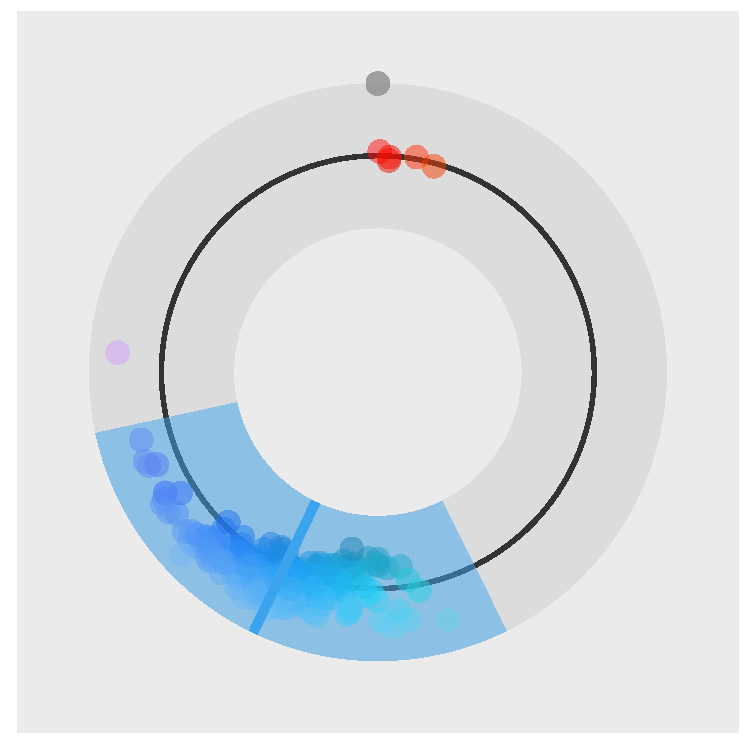
\includegraphics[width=\linewidth]{single_column.pdf}
% 	\caption{\textbf{A random visualization.} This is an example of a figure that spans only across one of the two columns.}
% 	\label{fig:column}
% \end{figure}

% On the other hand, \figurename~\ref{fig:whole} is an example of a figure that spans across the whole page (across both columns) of the report.

% % \begin{figure*} makes the figure take up the entire width of the page
% \begin{figure*}[ht]\centering 
% 	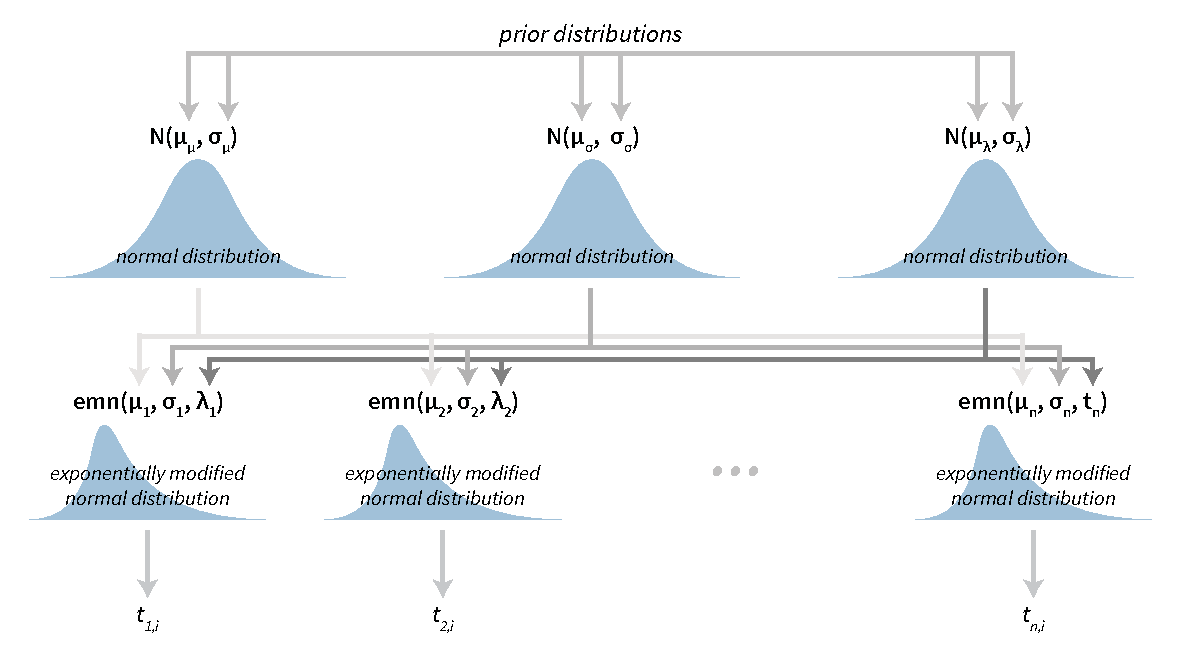
\includegraphics[width=\linewidth]{whole_page.pdf}
% 	\caption{\textbf{Visualization of a Bayesian hierarchical model.} This is an example of a figure that spans the whole width of the report.}
% 	\label{fig:whole}
% \end{figure*}


% \subsection*{Tables}

% Use the table environment to insert tables.

% \begin{table}[hbt]
% 	\caption{Table of grades.}
% 	\centering
% 	\begin{tabular}{l l | r}
% 		\toprule
% 		\multicolumn{2}{c}{Name} \\
% 		\cmidrule(r){1-2}
% 		First name & Last Name & Grade \\
% 		\midrule
% 		John & Doe & $7.5$ \\
% 		Jane & Doe & $10$ \\
% 		Mike & Smith & $8$ \\
% 		\bottomrule
% 	\end{tabular}
% 	\label{tab:label}
% \end{table}


% \subsection*{Code examples}

% You can also insert short code examples. You can specify them manually, or insert a whole file with code. Please avoid inserting long code snippets, advisors will have access to your repositories and can take a look at your code there. If necessary, you can use this technique to insert code (or pseudo code) of short algorithms that are crucial for the understanding of the manuscript.

% \lstset{language=Python}
% \lstset{caption={Insert code directly from a file.}}
% \lstset{label={lst:code_file}}
% \lstinputlisting[language=Python]{code/example.py}

% \lstset{language=R}
% \lstset{caption={Write the code you want to insert.}}
% \lstset{label={lst:code_direct}}
% \begin{lstlisting}
% import(dplyr)
% import(ggplot)

% ggplot(diamonds,
% 	   aes(x=carat, y=price, color=cut)) +
%   geom_point() +
%   geom_smooth()
% \end{lstlisting}

% %------------------------------------------------

% \section*{Results}

% Use the results section to present the final results of your work. Present the results in a objective and scientific fashion. Use visualisations to convey your results in a clear and efficient manner. When comparing results between various techniques use appropriate statistical methodology.

% \subsection*{More random text}

% This text is inserted only to make this template look more like a proper report. Lorem ipsum dolor sit amet, consectetur adipiscing elit. Etiam blandit dictum facilisis. Lorem ipsum dolor sit amet, consectetur adipiscing elit. Interdum et malesuada fames ac ante ipsum primis in faucibus. Etiam convallis tellus velit, quis ornare ipsum aliquam id. Maecenas tempus mauris sit amet libero elementum eleifend. Nulla nunc orci, consectetur non consequat ac, consequat non nisl. Aenean vitae dui nec ex fringilla malesuada. Proin elit libero, faucibus eget neque quis, condimentum laoreet urna. Etiam at nunc quis felis pulvinar dignissim. Phasellus turpis turpis, vestibulum eget imperdiet in, molestie eget neque. Curabitur quis ante sed nunc varius dictum non quis nisl. Donec nec lobortis velit. Ut cursus, libero efficitur dictum imperdiet, odio mi fermentum dui, id vulputate metus velit sit amet risus. Nulla vel volutpat elit. Mauris ex erat, pulvinar ac accumsan sit amet, ultrices sit amet turpis.

% Phasellus in ligula nunc. Vivamus sem lorem, malesuada sed pretium quis, varius convallis lectus. Quisque in risus nec lectus lobortis gravida non a sem. Quisque et vestibulum sem, vel mollis dolor. Nullam ante ex, scelerisque ac efficitur vel, rhoncus quis lectus. Pellentesque scelerisque efficitur purus in faucibus. Maecenas vestibulum vulputate nisl sed vestibulum. Nullam varius turpis in hendrerit posuere.

% Nulla rhoncus tortor eget ipsum commodo lacinia sit amet eu urna. Cras maximus leo mauris, ac congue eros sollicitudin ac. Integer vel erat varius, scelerisque orci eu, tristique purus. Proin id leo quis ante pharetra suscipit et non magna. Morbi in volutpat erat. Vivamus sit amet libero eu lacus pulvinar pharetra sed at felis. Vivamus non nibh a orci viverra rhoncus sit amet ullamcorper sem. Ut nec tempor dui. Aliquam convallis vitae nisi ac volutpat. Nam accumsan, erat eget faucibus commodo, ligula dui cursus nisi, at laoreet odio augue id eros. Curabitur quis tellus eget nunc ornare auctor.


%------------------------------------------------

% \section*{Discussion}
% ZAKLJUCEK PRVEGA DELA...
% Use the Discussion section to objectively evaluate your work, do not just put praise on everything you did, be critical and exposes flaws and weaknesses of your solution. You can also explain what you would do differently if you would be able to start again and what upgrades could be done on the project in the future.


%------------------------------------------------

% \section*{Acknowledgments}

% Here you can thank other persons (advisors, colleagues ...) that contributed to the successful completion of your project.


%----------------------------------------------------------------------------------------
%	REFERENCE LIST
%----------------------------------------------------------------------------------------
\bibliographystyle{unsrt}
\bibliography{report}


\end{document}